\documentclass[twoside,twocolumn]{report}

%\usepackage{blindtext} % Package to generate dummy text throughout this template 

\usepackage[sc]{mathpazo} 
\usepackage[T1]{fontenc} % Use 8-bit encoding that has 256 glyphs
\usepackage[utf8]{inputenc}% accents

\usepackage[english]{babel} % Language hyphenation and typographical rules

\usepackage[hmarginratio=1:1,top=20mm,columnsep=17pt]{geometry} % Document margins
\usepackage[hang, small,labelfont=bf,up,textfont=it,up]{caption} % Custom captions under/above floats in tables or figures
\usepackage{booktabs} % Horizontal rules in tables


\usepackage{enumitem} % Customized lists
\setlist[itemize]{noitemsep} % Make itemize lists more compact
\geometry{verbose,tmargin=2cm,bmargin=2.5cm,lmargin=2cm,rmargin=2cm}
\usepackage{abstract} % Allows abstract customization
\renewcommand{\abstractnamefont}{\normalfont\bfseries} % Set the "Abstract" text to bold
\renewcommand{\abstracttextfont}{\normalfont\small\itshape} % Set the abstract itself to small italic text

\usepackage{titlesec} % Allows customization of titles
\renewcommand\thesection{\Roman{section}} % Roman numerals for the sections
\renewcommand\thesubsection{\roman{subsection}} % roman numerals for subsections
\titleformat{\section}[block]{\large\scshape\centering}{\thesection.}{1em}{} % Change the look of the section titles
\titleformat{\subsection}[block]{\large}{\thesubsection.}{1em}{} % Change the look of the section titles

\usepackage{fancyhdr} % Headers and footers
\pagestyle{fancy} % All pages have headers and footers
\fancyhead{} % Blank out the default header
\fancyfoot{} % Blank out the default footer
\fancyhead[C]{Music regenerator   $\bullet$ November 2016 } % Custom header text
\fancyfoot[RO,LE]{\thepage} % Custom footer text

\usepackage{titling} % Customizing the title section

\usepackage{hyperref} % For hyperlinks in the PDF
\usepackage{amsmath} % Customizing the title section
\usepackage{graphicx,epstopdf}
\usepackage{mathtools}
\usepackage[colorinlistoftodos,prependcaption,textsize=tiny]{todonotes}
%----------------------------------------------------------------------------------------
%	TITLE SECTION
%----------------------------------------------------------------------------------------

\setlength{\droptitle}{-4\baselineskip} % Move the title up

\pretitle{\begin{center}\Huge\bfseries} % Article title formatting
\posttitle{\end{center}} % Article title closing formatting
\title{Music REgenerator } % Article title
\author{%
\textsc{Samuel Dupont}\\ %\thanks{A thank you or further information} \\[1ex] 
\textsc{Lucas Bourneuf}\\% Your name
%\normalsize Université du Maine \\ % Your institution
\normalsize \href{mailto:Samuel.dupont.etu@univ-lemans.fr}{Samuel.dupont.etu@univ-lemans.fr } 
}

\date{November 26, 2016 \\ Last update: \today}
\renewcommand{\maketitlehookd}{%
\begin{abstract}
\noindent 

This report is written to explicit the different parts of the music regenerator project. The global aim is to generate non random music using statistical tool which is listenable and sounds good. It's based on the decomposition of one or several musics in an index of probability of the note to play. This decomposition is achieved using Markov chain method.\\ The music is based on two main parameters which are the pitch of the note (the midi notation is used), and the note position. This result in the construction of two Markov chains one for the rhythm and one for the note. Both of them are for now independent and generate a music which is acceptable to hear let a big margin for improvements.  \\ \\
A part of this project is also dedicated to the transcription of music into MIDI format using pitch recognition algorithm and onset detection. It explores two methods of pitch reconignition one based on a modified cepstrum and another based on a modified autocorrelation method. The results are good for a part of the musical spectra however in the high frequency domain it becomes less effecting resulting in the wrong estimation of the played note.
\end{abstract}
}

%----------------------------------------------------------------------------------------

\begin{document}

% Print the title
\maketitle

\chapter{Dsp and audio algorithm for pitch recognition}
\section{Introduction}
In order to be able to convert a musical sample from a wav file for example, it needed to accurately determine the pitch of the different notes. This chapter will present two different methods based on the work of Philip McLeod \cite{mcleod2009fast}. There are based on the decomposition of the note into several smaller windows where the algorithm is applied, then the results of all the windows are reunified to achieve the final pitch estimation. \\
A first section will present the two different algorithms,  the second will explain the pre processing steps and then how to assemble the results. Next the evaluation of the methods will be discussed before the conclusion.\\
The figure \ref{input50} shows an input signal of 4024 points corresponding to midi 50 played with a piano used for the following figure.
\begin{figure}[h!]
	\centering
	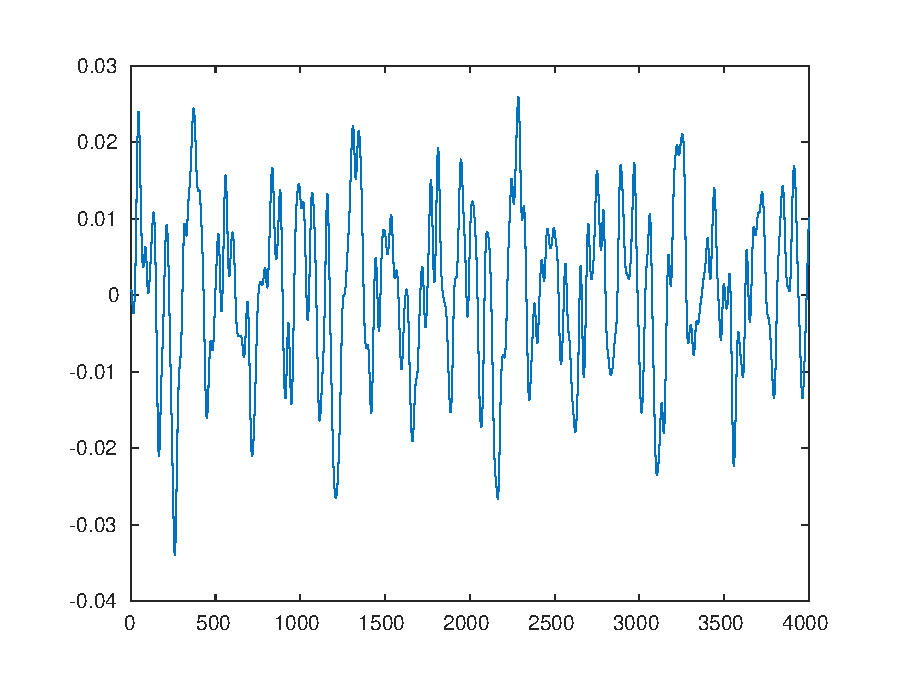
\includegraphics[width=260px]{./images/input_midi50.eps}
	\caption{Wav input midi 50, 4024 points}
	\label{input50}
\end{figure}
\section{SNAC function and modified cepstrum}
\subsection{SNAC algorithm}
The SNAC algorithm is based on autocorrelation, but the normalisation is done using the energy at each instant of calculation $\tau$ used for the autocorrelation. It's expressed by the following function:

\begin{equation}
	n'(\tau)=\frac{2 \sum_{j=0}^{W-1-\tau}x_j x_{j+\tau}}{\sum_{j=0}^{W-1-\tau}(x^2_j+ x^2_{j+\tau})},
\end{equation}
where $W$ is the length of the windows, $\tau$ the discretised instant and $x_j$ the sample to analyse.\\
The denominator as shown in the thesis \cite{mcleod2009fast} can be done in an iterative way:
\begin{equation}
\begin{split}
m'(\tau) & = \sum_{j=0}^{W-1-\tau}(x^2_j+ x^2_{j+\tau}),\\
		 & = m'(\tau-1)- x^2_{\tau-1}- x_{W-\tau},\\
\end{split}
\end{equation} 
with $m'(0)= 2 \sum_{j=0}^{W-1}x^2_j$.\\
\\
The figure \ref{SNACalgo50} shows an example of result from a SNAC function. It's  that a time domain signal centred around zero. It allows to define a peak between two zeros. The pitch of the signal is defined as the maximum peak, around n=300, thus the pitch is situated at $F_s/300$ which correspond to midi 50 as expected.
\begin{figure}[h!]
	\centering
	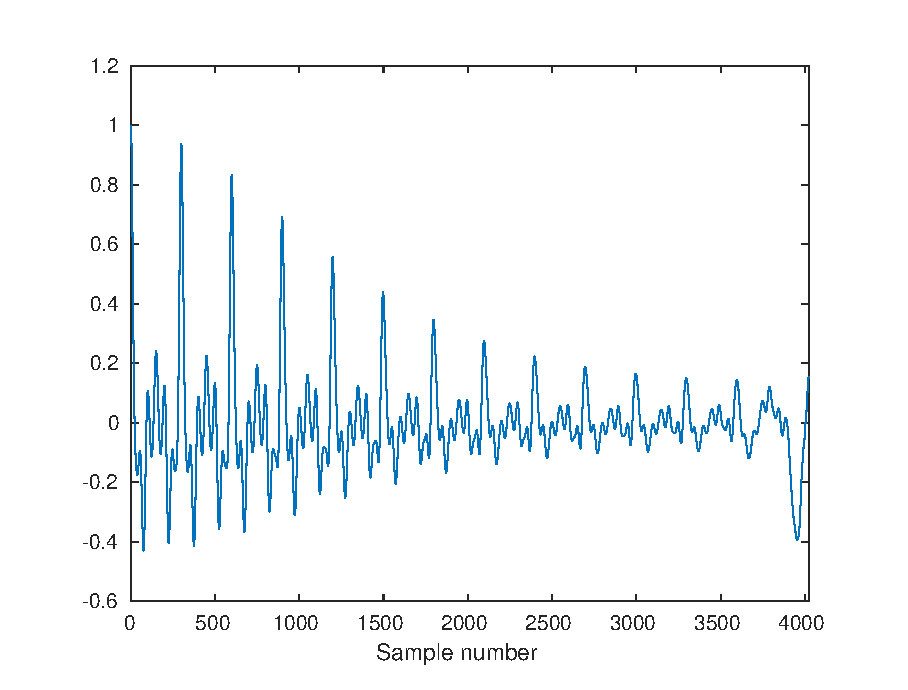
\includegraphics[width=260px]{./images/SNAC_functionR_4024pt_midi50.eps}
	\caption{Example of result for SNAC algorithm, midi 50, 4024 pt}
	\label{SNACalgo50}
\end{figure}
\subsection{Modified cepstrum}
The modified cepstrum come also from the thesis of P.McLeod \cite{mcleod2009fast}. It results of the addition of 1 in the $\log $ part of the cepstrum avoiding that the small values affect the result of the cepstrum.\\
The modified cepstrum is expressed as:
\begin{equation}
	mcep=\real{FFT(\log(1+abs(FFT(x))))}
\end{equation}
The figure \ref{Mcepalgo50} shows an example of result from a modified Cepstrum function. It's observed the same behaviour than the SNAC function, although there is a repetition of the half shape due to the FFT calculation.
\begin{figure}[h!]
	\centering
	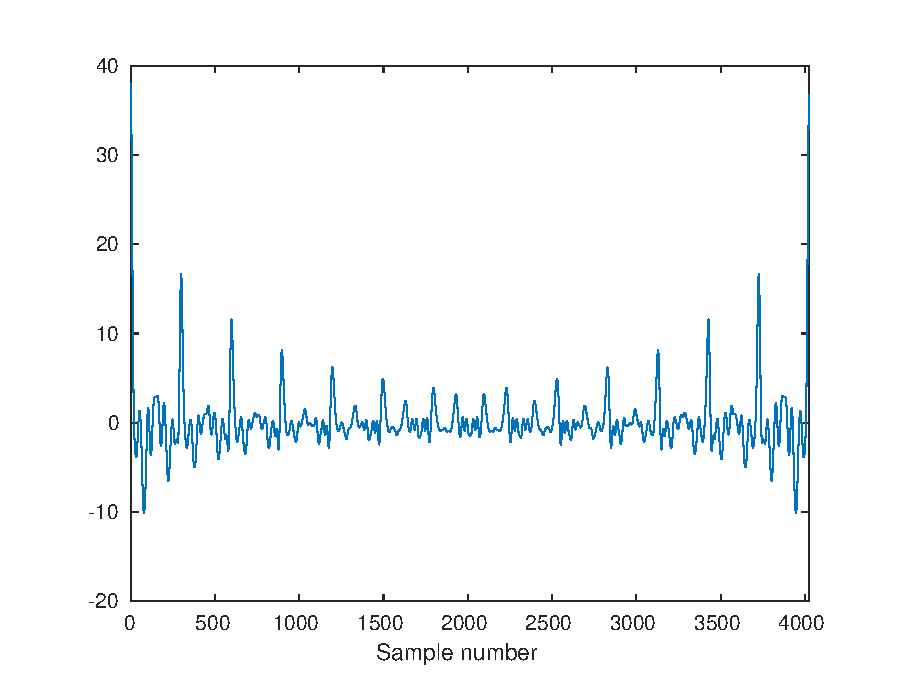
\includegraphics[width=260px]{./images/Mcepstrum_functionR_4024pt_midi50.eps}
	\caption{Example of result for modified Cepstrum algorithm, midi 50, 4024 pt}
	\label{Mcepalgo50}
\end{figure}
\section{Preconditioning the input signal }
\subsection{Window of signal}
Instead of using a rectangular window it's used a Hann window which reduce the contribution from the edges, the hann windows is shown on figure \ref{hann}. 
\begin{figure}[h!]
	\centering
	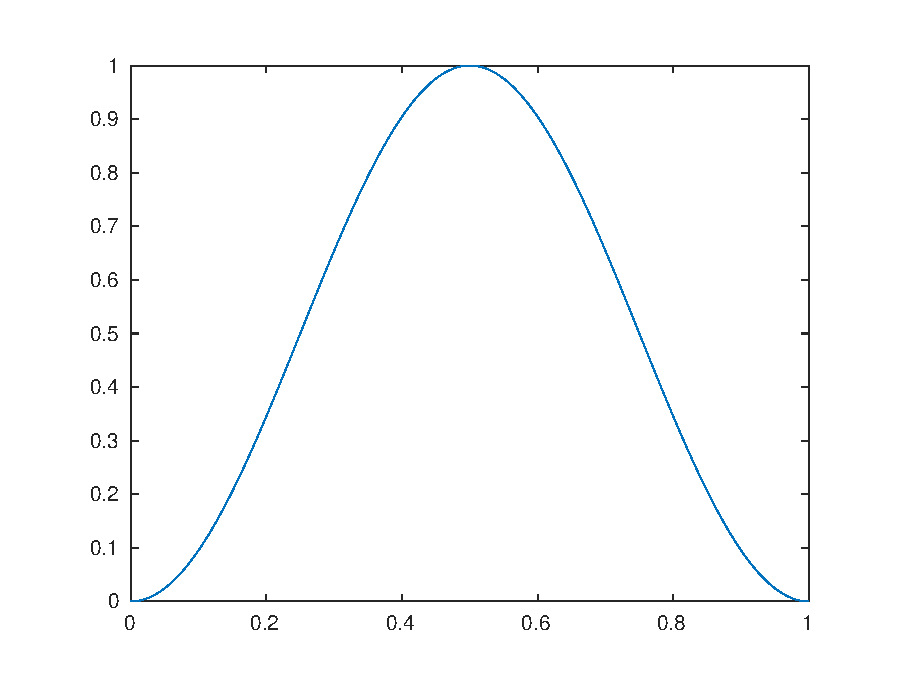
\includegraphics[width=260px]{./images/hann4024.eps}
	\caption{Hann windows used for preprocessing}
	\label{hann}
\end{figure}
\subsection{Outer medium ear filter }
The ears have a special frequency shape on the audio range (20Hz-20kHz), thus the loudness of the sound depend on the frequency. The figure \ref{loud} shows the perceived equal loudness (phone, in red) as function of the frequency and the level ($dB_{spl}$).\\
It's proposed in P.McLeod to make a filter simulating this effect using a yulewalk filter and a second order low pass Butterworth filter, the resulting filter is shown on figure \ref{mdouterfilt}.
\begin{figure}[h!]
	\centering
	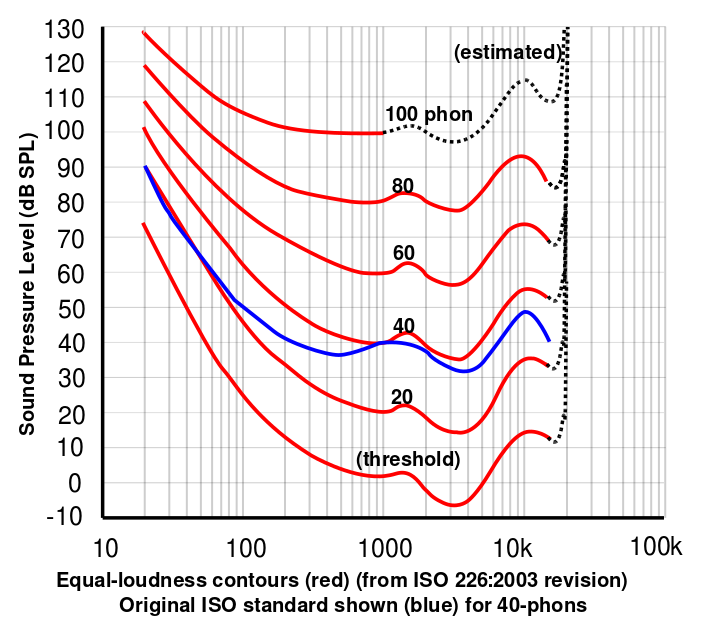
\includegraphics[width=260px]{./images/loudness.png}
	\caption{Perceived loudness of the sound}
	\label{loud}
\end{figure}
\begin{figure}[h!]
	\centering
	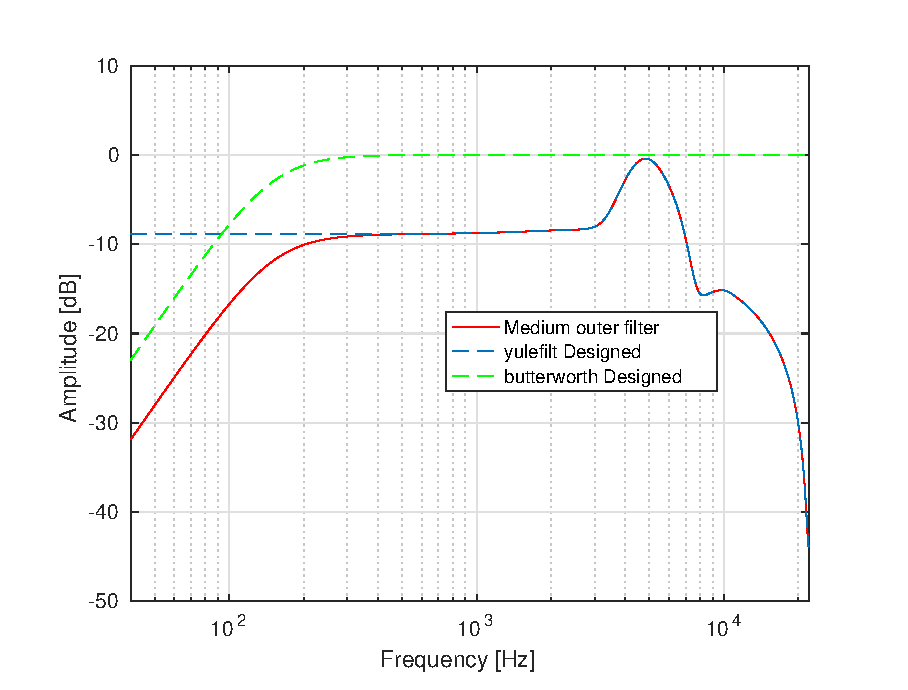
\includegraphics[width=260px]{./images/mdouterfilt.eps}
	\caption{Medium outer filter }
	\label{mdouterfilt}
\end{figure}
\subsection{Aggregate Lag Domain (ALD) }
\subsection{Peak picking method}
\todo{Do a graph recap of the algorithm}

\section{Assertion of both method.}
\chapter{Music note classification}

\chapter{Music regeneration }
\section{Conclusion}

%----------------------------------------------------------------------------------------
%	REFERENCE LIST
%--------------------------------------%
\begin{thebibliography}{99} % Bibliography - this is intentionally simple in this template



\bibitem{mcleod2009fast}{ McLeod\H Philip, \emph{Fast, accurate pitch detection tools for music analysis}, Academisch proefschrift, 2009 , University of Otago. Department of Computer Science}

\bibitem[\href{http://www.piano-midi.de/mendelssohn.htm}{http://www.piano-midi.de/mendelssohn.htm}]{site3}

%\newblock Assortative pairing and life history strategy - a cross-cultural
%  study.
%\newblock {\em Human Nature}, 20:317--330.
 
\end{thebibliography}--------------------------------------------------



%----------------------------------------------------------------------------------------

\end{document}
